% !TEX root = ./discrete_hydraulic_transients.tex

\documentclass[12pt]{article}
\usepackage{geometry}
 \geometry{
 a4paper,
 total={170mm,257mm},
 left=20mm,
 top=20mm,
 }
\usepackage{hyperref}
\usepackage{amsmath}
\usepackage{amsfonts}
\usepackage{xcolor}
\usepackage{verbatim}
\usepackage{tikz}
\usetikzlibrary{shapes.misc}
\usepackage{titlesec}

\setcounter{secnumdepth}{4}

\titleformat{\paragraph}
{\normalfont\normalsize\bfseries}{\theparagraph}{1em}{}
\titlespacing*{\paragraph}
{0pt}{3.25ex plus 1ex minus .2ex}{1.5ex plus .2ex}

\tikzset{cross/.style={cross out, draw=black, minimum size=2*(#1-\pgflinewidth), inner sep=0pt, outer sep=0pt},
%default radius will be 1pt. 
cross/.default={1pt}}

\newcommand{\pardiv}[3]{\frac{\partial^{#1} #2}{\partial #3^{#1}}}
\newcommand{\deriv}[3]{\frac{d^{#1} #2}{d #3^{#1}}}
 
\title{A discrete calculus approach to simulating hydraulic transients in pipe networks}
\author{Anthony O'Neill  \\
	Flite Software  \\
	}

\date{\today}
% Hint: \title{what ever}, \author{who care} and \date{when ever} could stand 
% before or after the \begin{document} command 
% BUT the \maketitle command MUST come AFTER the \begin{document} command! 
\begin{document}

\maketitle

\begin{abstract}
Typically hydraulic transients in pipe networks are simulated using either the method of characteristics (MOC) or the wave characteristics method (WCM). The WCM simplifies the calculations in order to decrease the computation cost at the expense of accuracy whereas the MOC offers higher spatial resolution but may require significantly more computational resources. The time step in the MOC may need to be very small in order to ensure the numerical stability of the solution which can have a significant impact on the run time for a simulation. This paper develops a discrete calculus approach to the problem of hydraulic transients in pipe networks which aims to maintain the flexibility of the WCM without compromising the accuracy that is obtained using the MOC. The scheme employed herein allows spatial and temporal discretisation to be refined as necessary without the need to alter pipe wave speeds in order to satisfy the Courant-Friedrich-Lewy (CFL) stability condition.
\end{abstract}

\section{Introduction} \label{sec:introduction}

Alterations to steady state pipe flow, such as valve closure, may cause severe pressure fluctuations throughout the system until a new steady state flow is recovered. This transient flow can have a significant impact on the design of piping networks as the system must be made sufficiently stronger to cope with sudden surges or drops in pressure. Pressure waves travel from the source of the disturbance at the speed of sound for the fluid medium usually being dissipated by viscous effects or by the geometry of the system. 

\subsection{Water hammer} \label{subsec:water_hammer}
Typically a time varying one-dimensional model for transient flow in closed conduits is constructed from the conservation of mass and momentum and Reynolds transport theorem (see chapter 2 of \cite{chaudhry14} for details). These equations govern either the pressure $p$ and velocity $V$ of the fluid or the piezometric head $H$ and the discharge $Q$ as functions of the spatial coordinate $x$ and time $t$. The flow is assumed to be slightly compressible and the conduit walls slightly deformable such that spatial variation of the fluid density $\rho$ and the conduit cross-sectional area $A$ are neglected. Thus the water hammer equations, in terms of $H$ and $Q$, are given by 
\begin{subequations}\label{governing_equations_discharge}
\begin{gather}
\pardiv{}{H}{t} + \frac{a^2}{g A} \pardiv{}{Q}{x} = C(x), \\
\pardiv{}{Q}{t} + g A \pardiv{}{H}{x} = \hat{R}(Q),
\end{gather}
where $g$ is the acceleration due to gravity, $a$ is the velocity of the pressure wave in an elastic conduit filled with a slightly compressible fluid, $C(x)$ is the known spatially varying consumption (flow into or out of the system) and $\hat{R}(Q)$ is a resistance term which specifies the pipe friction acting on the fluid. Typically the resistance term is taken to be 
\begin{equation}
\hat{R}(Q) = - \frac{f(Q) Q |Q|}{2 D A},
\end{equation} 
where $D$ is the conduit diameter and $f(Q)$ is the dimensionless Darcy-Weisbach friction factor which incorporates friction losses and is a function of the flow Reynolds number.
\end{subequations}
The velocity of the pressure wave in the conduit is determined by
\begin{align}
a^2 = \frac{\frac{K}{\rho}}{1 + \frac{DK}{eE}} = \frac{eEK}{\rho \left(eE + DK \right)},
\end{align}
where $K$ is the bulk modulus of elasticity for the fluid, $e$ is the thickness of the conduit walls and $E$ is the Young's modulus for the container material. The friction factor $f$ depends both upon the Reynold number of the flow and the relative roughness of the pipe. There are a number of different empirical equations for determining the friction factor $f$, such as the implicit Colebrook-White equation {\color{red}(this should be looked at in more detail as there are a number of different options)}. 

Equations \eqref{governing_equations_discharge} are the basic equations governing transient flow in a pipe, terms can be added or modified to account for more complex phenomena such as pipe inclination or a more exotic friction term (see Wylie \& Streeter for details\cite{streeter78}). The numerical solution of \eqref{governing_equations_discharge} may be approached in a number of different ways including the method of characteristics, the wave characteristics method, explicit finite-difference schemes (and variations such as Lax-Wendroff and MacCormack), Implicit finite-difference schemes and spectral methods. 

In general the flows we will be modelling exist in complex networks of interconnected components such as pipes, valves and pumps which may be modelled as resistances to the flow through the particular component. Although these networks exist as three-dimensional structures we may simplify our analysis by considering these components to be connected one-dimensional objects. This approach presents challenges for us in modelling the connections between components but significantly reduces the complexity when solving the system numerically. This approach is analogous to the idea of the circuit diagram often used in electrical engineering and will presented in a similar way.  
 


\section{Discrete calculus} \label{sec:discrete_calculus}

We wish to describe the temporal variation of the volume flow rate $Q$ and the head $H$ in a one-dimensional domain. This presents us with a bit of problem when it comes to determining flows in networks as connections between more than two pipes/components aren't one-dimensional. One way to approach this difficulty is by considering a discrete calculus \cite{grady10} formulation for the governing equations.

\subsection{Discrete calculus formulation}\label{subsec:discrete_calculus_steady}

The discrete calculus approach has the advantage of directly using the network structure to calculate the derivatives. In the discrete calculus formulation a network is represented as a graph (1-complex) where the edges (1-cells) represent pipes/components and the nodes (0-cells) represent connections and boundaries. The edges of the graph consist of ordered pairs of nodes which define the orientation of the edge. The boundary of each edge is comprised of the union of nodes and the intersection of any two edges is either empty or a boundary element of both edges. 

Flow passing through an edge in the same direction as its orientation is considered positive while flow in the opposite direction is considered negative. We will consider edges that are oriented but not directed since flow is permitted in both directions. An edge consists of two nodes (labelled $\sigma_1$ and $\sigma_2$) and the orientation may be defined by an ordering of these nodes as the list $\tau = \{ \sigma_1, \sigma_2 \}$. A node is considered to have two orientations ("sourceness" and "sinkness") but by convention all nodes will be given the same orientation, "sourceness", so that the negative end of an edge will not be coherent with the orientation of a node.   

\begin{figure}
\centering
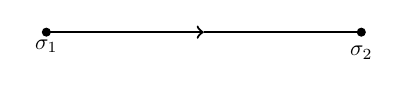
\begin{tikzpicture}[scale=1, every node/.style={scale=0.8}] 
\node[anchor=north] at (3,0) {$\sigma_1$};
\draw[fill=black] (3,0) circle (0.05cm);
\node[anchor=north] at (7,-0.08) {$\sigma_2$};
\draw[fill=black] (7,0) circle (0.05cm);
\draw[thick, ->] (3,0) -- (5,0);
\draw[thick] (5,0) -- (7,0);
\end{tikzpicture} 
\caption{The edge points from $\sigma_1$ to $\sigma_2$; flow from $\sigma_1$ to $\sigma_2$ is considered positive.}
\label{fig:edge_orientation}
\end{figure}

\subsubsection{Incidence matrix}

The structure of a graph (network) may be represented algebraically via an incidence matrix. The incidence matrix $\mathbf{K}^T$ encodes which edges are incident to which nodes in the graph and is defined as 
\begin{align}
K_{ij}=
\begin{cases}
\hspace{0.3cm} 0 \hspace{0.5cm} \text{if } \sigma_j \text{ is not on the boundary of } e_i, \\
+1 \hspace{0.5cm} \text{if } \sigma_j \text{ is coherent with the orientation of } e_i,\\
-1 \hspace{0.5cm} \text{if } \sigma_j \text{ is not coherent with the orientation of } e_i,
\end{cases}
\end{align}
where $e_i$ is the label of an edge in the graph. For a graph the incidence matrix $\mathbf{K}^T$ is an $n \times m$ matrix (where $n$ is the number of nodes and $m$ is the number of edges). For example the graph shown in figure \ref{fig:example_network} has 
\begin{align*}
\mathbf{K} = \begin{bmatrix}
1 & -1 & 0 & 0 & 0 \\
0 & 1 & -1 & 0 & 0 \\
0 & 0 & 1 & -1 & 0 \\
0 & 0 & 1 & 0 & -1 
\end{bmatrix},
\end{align*}
such that the incidence matrix is given by 
\begin{align*}
\mathbf{K}^T = \begin{bmatrix}
1 & 0 & 0 & 0 \\ 
-1 & 1 & 0 & 0 \\
0 & -1 & 1 & 1 \\
0 & 0 & -1 & 0 \\
0 & 0 & 0 & -1
\end{bmatrix}.
\end{align*}

\begin{figure}
\centering
\begin{tikzpicture}[scale=1, every node/.style={scale=0.8}] 
\node[anchor=north] at (3,-0.08) {$\sigma_1$};
\draw[fill=black] (3,0) circle (0.05cm);
\node[anchor=north] at (5,-0.08) {$\sigma_2$};
\draw[fill=black] (5,0) circle (0.05cm);
\node[anchor=north] at (7,-0.08) {$\sigma_3$};
\draw[fill=black] (7,0) circle (0.05cm);
\node[anchor=north] at (9,-0.08) {$\sigma_4$};
\draw[fill=black] (9,0) circle (0.05cm);
\node[anchor=south] at (7,2+0.08) {$\sigma_5$};
\draw[fill=black] (7,2) circle (0.05cm);
\draw[thick, ->] (3,0) -- (4,0);
\draw[thick] (4,0) -- (5,0);
\draw[thick, ->] (5,0) -- (6,0);
\draw[thick] (6,0) -- (7,0);
\draw[thick, ->] (7,0) -- (8,0);
\draw[thick] (8,0) -- (9,0);
\draw[thick, ->] (7,0) -- (7,1);
\draw[thick] (7,1) -- (7,2);
\node[anchor=south] at (4,0.08) {$e_1$};
\node[anchor=south] at (6,0.08) {$e_2$};
\node[anchor=south] at (8,0.08) {$e_3$};
\node[anchor=west] at (7+0.08,1) {$e_4$};
\end{tikzpicture} 
\caption{An example graph with 5 nodes and 4 edges.}
\label{fig:example_network}
\end{figure}

\subsubsection{Chains}

In order to define a domain of integration on the graph we must define a 1-chain. A 1-chain is an $m$-tuple of scalars which assigns a coefficient to each edge where $m$ is the number of distinct edges in the graph. A 1-chain is represented by a column vector of size $m$ with zeros in the entries corresponding to edges not included in the chain. A 1-chain may be viewed as an indicator vector representing a set of edges i.e. $\mathbf{\tau}_1 = [1, 1, 0, 0]^T$ represents the set of edges $\{ e_1, e_2 \}$. Generally a 1-chain $\mathbf{\tau}_1$ may be expressed as 
\begin{align}
\mathbf{\tau}_1 =  \sum_{i=1}^m a^i \mathbf{e}_i, \hspace{0.5cm} a^i \in \mathbb{R},
\end{align}
where the sign of $a^i$ indicates the orientation and $\mathbf{e}_i$ are basis vectors for each edge. 

The incidence matrix $\mathbf{K}^T$ maps 1-chains into their corresponding boundary elements. In other words when $\mathbf{K}^T$ is applied to a 1-chain (edge chain) the result is a 0-chain (node chain) i.e. $\mathbf{\tau}_0 = \mathbf{K}^T \mathbf{\tau}_1$. The chain $\mathbf{\tau}_0$ represents the oriented set of nodes on the boundary of the edges represented by $\mathbf{\tau}_1$. For example for the nodes on the boundary of edges $e_1$ and $e_2$ we have
\begin{align*}
\mathbf{\tau}_0 = \mathbf{K}^T \begin{bmatrix}
1 \\ 1 \\ 0 \\ 0
\end{bmatrix} = \begin{bmatrix}
1 \\ 0 \\ -1 \\ 0 \\ 0
\end{bmatrix},
\end{align*}
which corresponds to the nodes $\sigma_1$ and $\sigma_3$ as expected. For the boundary of the entire graph we have 
\begin{align*}
\mathbf{\tau}_0 = \mathbf{K}^T \begin{bmatrix}
1 \\ 1 \\ 1 \\ 1
\end{bmatrix} = \begin{bmatrix}
1 \\ 0 \\ 1 \\ -1 \\ -1
\end{bmatrix},
\end{align*}
where we see that join points ($\sigma_3$) are considered part of the boundary set. The incidence matrix $\mathbf{K}^T$ provides both a representation of the topology of the graph and the boundary operator. 

\subsubsection{Discrete forms}

We may define a vector space that locally maps 1-chains to scalars at each edge in the graph, called 1-cochains. A 1-cochain may be viewed as a function defined on the domain of edges. We represent a 1-cochain as an $m \times 1$ column vector $\mathbf{c}^1$ where the sign of each coefficient indicates the orientation. We can define integration as the pairing (inner product) of a 1-chain with a 1-cochain,
$[\![ \mathbf{c}^1, \mathbf{\tau}_1 ]\!] = \mathbf{c}^1 \cdot \mathbf{\tau}_1$, producing a scalar quantity. 

\subsubsection{Metric tensor}

Given a set of basic chains $\sigma_i$ we may define a metric tensor 
\begin{align*}
g_{ij} = \langle \sigma_i, \sigma_j \rangle.
\end{align*}
Typically in the discrete setting, the basis set of edges is defined to be orthogonal such that $g_{ij}=0$ for $i \neq j$. The metric tensor thus represented by the $m \times m$ diagonal matrix $\mathbf{G}$ where $\mathbf{G}=\text{diag}(g_{ii})$. Converting a 1-chain into its equivalent 1-cochain consists of a simple scaling of the chain coefficients $\mathbf{c}^1 = \mathbf{G} \mathbf{\tau}_1$.


\section{Component networks} \label{sec:component_networks}

In order to model the flow network we shall suppose that a generic components is represented by an edge and the connectivity of those components by nodes. A general component, as shown in \ref{fig:transient_element}, has an average mass flow rate defined at the center of the element and nodal pressure at either end. The mass flow rate is assumed to vary along the component so that in general the mass flow rate at each end does not equal the average mass flow rate in the component. 

\begin{figure}
\centering
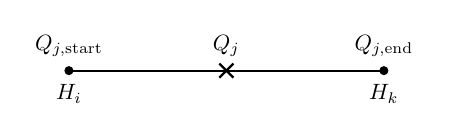
\begin{tikzpicture}[scale=1, every node/.style={scale=0.8}] 
%\draw[step=1cm,color=gray] (3,0) grid (7,3);
\node[anchor=north] at (3,-0.08) {$H_i$};
\draw[fill=black] (3,0) circle (0.05cm);
\node[anchor=south] at (5,0.08) {$Q_j$};
\draw[thick] (5,0) node[cross=4pt] {};
\node[anchor=north] at (7,-0.08) {$H_k$};
\draw[fill=black] (7,0) circle (0.05cm);
\draw[thick] (3,0) -- (7,0);
\node[anchor=south] at (3,0.08) {$Q_{j,\text{start}}$};
\node[anchor=south] at (7,0.08) {$Q_{j,\text{end}}$};
\end{tikzpicture} 
\caption{A general component $j$ with an average volume flow rate $Q_j$ and nodal heads $H_i$ and $H_k$.}
\label{fig:transient_element}
\end{figure}

For simplicity we shall suppose that the variation in flow rate in an element is linear so that by combining multiple elements we will be able to approximate the true variation and improve this approximation by increasing the number of elements used in the model. Using first order forward and backward differences we have 
\begin{align}
\pardiv{}{Q}{x} \bigg\vert_{j,\text{end}} =& \frac{Q_{j,\text{end}} - Q_j}{\frac{1}{2}L_j}, \\
\pardiv{}{Q}{x} \bigg\vert_{j,\text{start}} =& \frac{Q_j - Q_{j,\text{start}}}{\frac{1}{2}L_j}. 
\end{align} 
Also we have 
\begin{align}
\pardiv{}{Q}{x} \bigg\vert_{j,\text{end}} =& -\frac{gA_j}{a_j^2} \pardiv{}{H_k}{t}, \\
\pardiv{}{Q}{x} \bigg\vert_{j,\text{start}} =& -\frac{gA_j}{a_j^2} \pardiv{}{H_i}{t}, 
\end{align}
therefore
\begin{align}
Q_{j,\text{end}} =& Q_j - \frac{gA_j L_j}{2 a_j^2} \pardiv{}{H_k}{t}, \\
Q_{j,\text{start}} =& Q_j + \frac{gA_j L_j}{2 a_j^2} \pardiv{}{H_i}{t}.
\end{align}
Here $L_j$, $A_j$ and $a_j$ are the component length, area and wavespeed respectively. Conservation of mass requires that the sum of the flow rates into a node equals zero. An example is useful for demonstrating how this condition can be enforced at each node. 

\begin{figure}
\centering
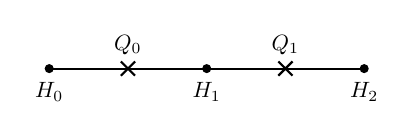
\begin{tikzpicture}[scale=1, every node/.style={scale=0.8}] 
%\draw[step=1cm,color=gray] (3,0) grid (7,3);
\node[anchor=north] at (3,-0.08) {$H_0$};
\draw[fill=black] (3,0) circle (0.05cm);
\node[anchor=south] at (4,0.08) {$Q_0$};
\draw[thick] (4,0) node[cross=4pt] {};
\node[anchor=north] at (5,-0.08) {$H_1$};
\draw[fill=black] (5,0) circle (0.05cm);
\node[anchor=south] at (6,0.08) {$Q_1$};
\draw[thick] (6,0) node[cross=4pt] {};
\node[anchor=north] at (7,-0.08) {$H_2$};
\draw[fill=black] (7,0) circle (0.05cm);
\draw[thick] (3,0) -- (5,0);
\draw[thick] (5,0) -- (7,0);
\end{tikzpicture} 
\caption{A (very) simple example network.}
\label{fig:discrete_calculus_example_network}
\end{figure}

Consider the very simple example network shown in figure \ref{fig:discrete_calculus_example_network} the continuity condition at each node is given by 
\begin{align*}
\begin{bmatrix}
Q_{0,\text{start}} \\ Q_{1,\text{start}} - Q_{0,\text{end}} \\ -Q_{1,\text{end}}
\end{bmatrix} = \begin{bmatrix}
Q_0 + \frac{gA_0 L_0}{2 a_0^2} \pardiv{}{H_0}{t} \\
Q_1 + \frac{gA_1 L_1}{2 a_1^2} \pardiv{}{H_1}{t} - Q_0 + \frac{gA_0 L_0}{2 a_0^2} \pardiv{}{H_1}{t} \\
-Q_1 + \frac{gA_1 L_1}{2 a_1^2} \pardiv{}{H_2}{t}
\end{bmatrix} = \mathbf{C},
\end{align*}
where $\mathbf{C}$ is the vector of nodal consumptions, which may be written as
\begin{align*}
\mathbf{K}^T \mathbf{Q} + \begin{bmatrix}
\frac{gA_0 L_0}{2 a_0^2} & 0 & 0 \\
0 & \frac{gA_0 L_0}{2 a_0^2} + \frac{gA_1 L_1}{2 a_1^2} & 0 \\
0 & 0 & \frac{gA_1 L_1}{2 a_1^2}
\end{bmatrix}
\pardiv{}{\mathbf{H}}{t} = \mathbf{C}.
\end{align*}

Let $\mathbf{K}_+$ be the matrix which contains a '1' in an entry only if $\mathbf{K}$ contains '1' in the same entry (otherwise 0) and let $\mathbf{K}_-$ be the matrix which contains a '1' in an entry only if $\mathbf{K}$ contains a '-1', for this example network 
\begin{align*}
\mathbf{K} = \begin{bmatrix}
1 & -1 & 0 \\
0 & 1 & -1
\end{bmatrix}
\end{align*}
therefore
\begin{align*}
\mathbf{K}_+ = \begin{bmatrix}
1 & 0 & 0 \\
0 & 1 & 0
\end{bmatrix}
\hspace{0.5cm} \text{and} \hspace{0.5cm} \mathbf{K}_- = \begin{bmatrix}
0 & 1 & 0 \\
0 & 0 & 1
\end{bmatrix}.
\end{align*}
Using these definitions we may write the discrete continuity equation as 
\begin{align}\label{discrete_continuity_eqn}
\boxed{\mathbf{K}^T \mathbf{Q} + \mathbf{D} \pardiv{}{\mathbf{H}}{t} = \mathbf{C},}
\end{align}
where 
\begin{align*}
\mathbf{D} = \mathbf{K}_+^T \mathbf{M} \mathbf{K}_+ + \mathbf{K}_-^T \mathbf{M} \mathbf{K}_-
\end{align*}
and
\begin{align*}
\mathbf{M} = \text{diag}\left( \frac{gA_j L_j}{2 a_j^2}\right),
\end{align*}
where typically $M_{j,j} = 0$ when component $j$ is not a pipe.

For a network with $N_n$ nodes and $N_c$ components we require $N_n + N_c$ equations in order to the determine the flow rates and heads in the network. The system \eqref{discrete_continuity_eqn} gives us $N_n$ equations for the conservation of mass at each node so we still require $N_c$ additional equations in order to fully specify the system. 

\subsection{Component equations}

In order to maintain generality we shall specify the momentum equation in each edge in terms of a general resistance $\mathbf{R}$, which is specified for each particular type of component, such that 
\begin{align}\label{discrete_momentum_eqn}
\boxed{ \mathbf{B} \pardiv{}{\mathbf{Q}}{t}  = \mathbf{R}(\mathbf{Q}, \mathbf{K} \mathbf{H}),}
\end{align}
or in component form
\begin{align}
B_{j,j} \pardiv{}{Q_j}{t} = R_j( Q_j, \Delta H_j ).
\end{align}
The diagnoal matrix $\mathbf{B}$ is a matrix of coefficients, this allows us some flexibility when specifying the momentum equation, typically $B_{j,j} = 1$.
Specifying the resistance term in this way allows for greater flexibility in defining components. The most obvious component that we might consider is a pipe, from the Darcy-Weisbach equation we have
\begin{align}
\frac{\Delta H}{L} = \frac{f Q^2}{2 g D A^2} \implies \frac{f Q^2}{2 D A} - \frac{g A \Delta H}{L} = 0,
\end{align}
where $f = f(Q)$ is the friction factor. This means we may define a resistance term of the form
\begin{align}\label{pipe_resistance}
\boxed{ R_j = - \frac{f(Q_j)Q_j|Q_j|}{2 D_j A_j} + \frac{g A_j}{L_j} \Delta H_j. }
\end{align}
This is the correct form of the resistance term as in the continuous equation we have
\begin{align*}
\pardiv{}{Q}{t} = \hat{R}(Q) - g A \pardiv{}{H}{x} = R( Q, \partial H).
\end{align*}


The discrete equations \eqref{discrete_continuity_eqn} and \eqref{discrete_momentum_eqn}, when supplemented with appropriate boundary conditions, allow the flow rates and heads to be determined throughout the system. 


\section{Steady state solver} \label{sec:steady_state} 

In the absence of transients the discrete continuity equation \eqref{discrete_continuity_eqn} reduces to 
\begin{align}\label{discrete_steady_continuity_eqn}
\boxed{\mathbf{K}^T \mathbf{Q} = \mathbf{C}}
\end{align} 
and \eqref{discrete_momentum_eqn} reduces to 
\begin{align}\label{discrete_steady_momentum_eqn}
\boxed{\mathbf{R}(\mathbf{Q}, \mathbf{K} \mathbf{H}) = \mathbf{0} .}
\end{align}
We wish to solve \eqref{discrete_steady_continuity_eqn} along with the nonlinear momentum equations \eqref{discrete_steady_momentum_eqn}.

\subsection{Newton iteration}

Due to the nonlinear nature of \eqref{discrete_momentum_eqn} it is necessary to perform Newton iteration in order to converge to a solution. Let us split the flow rate and head vectors into a known/guessed part and a correction such that $\mathbf{Q} = \mathbf{Q}^g + \mathbf{Q}^c$ and $\mathbf{H} = \mathbf{H}^g + \mathbf{H}^c$ then 
\begin{align*}
\mathbf{R}(\mathbf{Q}, \mathbf{K} \mathbf{H}) \approx \mathbf{R}(\mathbf{Q}^g, \mathbf{K} \mathbf{H}^g ) + \pardiv{}{\mathbf{R}}{\mathbf{Q}} \Bigg\vert_{\mathbf{Q}^g} \mathbf{Q}^c + \pardiv{}{\mathbf{R}}{\mathbf{K} \mathbf{H}} \Bigg\vert_{\mathbf{K} \mathbf{H}^g} \mathbf{K} \mathbf{H}^c.
\end{align*}
The continuity equation \eqref{discrete_steady_continuity_eqn} is now given by
\begin{align}\label{discrete_steady_continuity_eqn_newton}
\mathbf{K}^T \mathbf{Q}^c = \mathbf{C} - \mathbf{K}^T \mathbf{Q}^g,
\end{align}
and the momentum equation \eqref{discrete_steady_momentum_eqn} is given by
\begin{align}\label{discrete_steady_momentum_eqn_newton}
- \pardiv{}{\mathbf{R}}{\mathbf{K} \mathbf{H}} \Bigg\vert_{\mathbf{K} \mathbf{H}^g} \mathbf{K} \mathbf{H}^c - \pardiv{}{\mathbf{R}}{\mathbf{Q}} \Bigg\vert_{\mathbf{Q}^g} \mathbf{Q}^c  = \mathbf{R}(\mathbf{Q}^g, \mathbf{K} \mathbf{H}^g).
\end{align}
These equations may be combined into a single system of the form
\begin{align}\label{discrete_steady_system}
\begin{bmatrix}
\mathbf{K}^T & \mathbf{0} \\
-\mathbf{J} & -\mathbf{G}
\end{bmatrix} 
\begin{bmatrix}
\mathbf{Q}^c \\ \mathbf{H}^c
\end{bmatrix} = \begin{bmatrix}
\mathbf{C} - \mathbf{K}^T \mathbf{Q}^g \\
\mathbf{R}(\mathbf{Q}^g, \mathbf{K} \mathbf{H}^g)
\end{bmatrix},
\end{align}
where $\mathbf{J} = \pardiv{}{\mathbf{R}}{\mathbf{Q}} \big\vert_{\mathbf{Q}^g}$ is the flow Jacobian matrix and $\mathbf{G} = \pardiv{}{\mathbf{R}}{\mathbf{K} \mathbf{H}} \big\vert_{\mathbf{K} \mathbf{H}^g} \mathbf{K}$. Boundary conditions specifying either the head or consumption at a node will modify this system of equations. 


\subsubsection{An example of the discrete calculus approach}

Consider the simple network shown in figure \ref{fig:discrete_calculus_example_network} which has $\mathbf{Q} = [Q_0, Q_1]^T$ and $\mathbf{H} = [H_0, H_1, H_2]^T$, along with
\begin{align*}
\mathbf{K} = \begin{bmatrix}
1 & -1 & 0 \\
0 & 1 & -1
\end{bmatrix}
\hspace{0.5cm} \text{and} \hspace{0.5cm} \mathbf{K}^T = \begin{bmatrix}
1 & 0  \\
-1 & 1 \\
0 & -1
\end{bmatrix}.
\end{align*}
We can see how the matrix product 
\begin{align*}
\mathbf{K}^T \mathbf{Q} = \begin{bmatrix}
1 & 0  \\
-1 & 1 \\
0 & -1
\end{bmatrix} \begin{bmatrix}
Q_0 \\ Q_1
\end{bmatrix} = \begin{bmatrix}
Q_0 \\ Q_1 - Q_0 \\ -Q_1
\end{bmatrix} = \mathbf{C}
\end{align*}
enforces that the sum of the flow rates into a node is equal to the consumption at that node. 

The system of equations (without boundary conditions) \eqref{discrete_steady_system} is given by
\begin{align*}
\begin{bmatrix}
1 & 0 & 0 & 0 & 0 \\
-1 & 1 & 0 & 0 & 0 \\
0 & -1 & 0 & 0 & 0 \\
-\pardiv{}{R}{Q}\big\vert_{Q_0^g} & 0 & -\pardiv{}{R}{\Delta H}\big\vert_{H_0^g - H_1^g} & \pardiv{}{R}{\Delta H}\big\vert_{H_0^g - H_1^g} & 0 \\
0 & -\pardiv{}{R}{Q}\big\vert_{Q_1^g} & 0 & -\pardiv{}{R}{\Delta H}\big\vert_{H_1^g - H_2^g} & \pardiv{}{R}{\Delta H}\big\vert_{H_1^g - H_2^g}
\end{bmatrix} \begin{bmatrix}
Q_0^c \\ Q_1^c \\ H_0^c \\ H_1^c \\ H_2^c
\end{bmatrix} = \begin{bmatrix}
C_0 - Q_0^g \\ 
C_1 - Q_1^g + Q_0^g \\ 
C_2 + Q_1^g \\ 
R\left(Q_0^g, H_0^g - H_1^g \right) \\ 
R\left(Q_1^g, H_1^g - H_2^g \right)
\end{bmatrix}.
\end{align*}
If we wished to specify head boundary conditions ($H_0 = H_{known} = 20$) at the first node and ($H_2 = P_{atm} / \rho g = 101325 / (999.7 \cdot 9.80665) = 10.33537514$) we would modify the system of equations to be 
\begin{align*}
\begin{bmatrix}
0 & 0 & 1 & 0 & 0 \\
-1 & 1 & 0 & 0 & 0 \\
0 & 0 & 0 & 0 & 1 \\
-\pardiv{}{R}{Q}\big\vert_{Q_0^g} & 0 & -\pardiv{}{R}{\Delta H}\big\vert_{H_0^g - H_1^g} & \pardiv{}{R}{\Delta H}\big\vert_{H_0^g - H_1^g} & 0 \\
0 & -\pardiv{}{R}{Q}\big\vert_{Q_1^g} & 0 & -\pardiv{}{R}{\Delta H}\big\vert_{H_1^g - H_2^g} & \pardiv{}{R}{\Delta H}\big\vert_{H_1^g - H_2^g}
\end{bmatrix} \begin{bmatrix}
Q_0^c \\ Q_1^c \\ H_0^c \\ H_1^c \\ H_2^c
\end{bmatrix} = \begin{bmatrix}
H_{known} - H_0^g \\ 
C_1 - Q_1^g + Q_0^g \\ 
\left( P_{atm} / \rho g \right) - H_2^g \\ 
R\left(Q_0^g, H_0^g - H_1^g \right) \\ 
R\left(Q_1^g, H_1^g - H_2^g \right)
\end{bmatrix}.
\end{align*}
The system of equations is then solved for the corrections, $\mathbf{Q}^c$ and $\mathbf{H}^c$, these are then used to update the guess $\mathbf{Q}^g \rightarrow \mathbf{Q}^g + \mathbf{Q}^c $ and $\mathbf{H}^g \rightarrow \mathbf{H}^g + \mathbf{H}^c $ and then process is repeated until the corrections are sufficiently small. Calculating the above example with two resistances being perfectly smooth pipes of lengths $L_0 = 100$m, $L_1 = 200$m and diameters $D_0=D_1=50$mm, with $C_1=0$, we obtain the solution $\mathbf{Q} = [0.00239623, 0.00239623]^T$ and $\mathbf{H} = [20, 16.77845838, 10.33537514]^T$. For such a simple example the system of equations is equivalent to the finite-difference form however for more complex networks, with multiple branches, the discrete calculus formulation allows the continuity condition to be satisfied without adding an additional constraint. 

\subsection{Resistances}

Each particular component in the network will have a different resistance term and different models of the same component may also produce different resistances. The typical resistance term for pipes is based on the Darcy-Weisbach equation and is shown in \eqref{pipe_resistance}. We will now outline some other resistance terms for common components. 

\subsubsection{Valves}

A valve has a discharge relationship defined by 
\begin{align}
Q = C_d A_v \sqrt{2 g \Delta H},
\end{align}
where $C_d$ is the discharge coefficient and $A_v$ is the valve opening area. Therefore 
\begin{align}
\Delta H = \frac{Q^2}{2g\left(C_d A_v \right)^2} = \frac{k Q^2}{2 g A^2} \implies \frac{k Q^2}{2A} - g A \Delta H = 0,
\end{align}
where $A$ is the cross-sectional area and $k$ is the loss coefficient which varies depending upon the percentage opening of the valve. This means that the resistance term for valves may be written as
\begin{align}
R_j = - \frac{k_j Q_j|Q_j| }{2 A_j} + g A_j \Delta H_j.
\end{align}
Alternatively we could write this resistance as 
\begin{align} \label{valve_resistance}
    \boxed{ R_j = - \frac{Q_j|Q_j| }{2 A_j} + k_j^{-1} g A_j \Delta H_j, }
\end{align}
but we must remember that in this form the transient coefficient in the matrix $\mathbf{B}$ is given by
\begin{align}
    \boxed{ B_{j,j} = k_j^{-1}. }
\end{align}
The loss coefficient $k$ may be determined from the discharge coefficient and the valve opening area using the relation 
\begin{align}
k = \frac{A^2}{\left(C_d A_v \right)^2} \implies k^{-1} = \frac{\left(C_d A_v \right)^2}{A^2} = k^{-1}(\tau),
\end{align}
where $\tau$ is the valve opening ratio. Writing the resistance function in the form \eqref{valve_resistance}, using $k^{-1}$, is more numerically stable as when the valve is fully closed, $A_v = 0$, $k \to \infty$ but $k^{-1} = 0$.

For example suppose we have a single valve resistance element with $H_0 = 20$, $H_1 = P_{atm} / \rho g$ with $k = 7$ and diameter $D = 50$mm. Then 
\begin{align}
Q =& \sqrt{\frac{2gA^2 \Delta H}{k}} = \pi D^2 \sqrt{\frac{g \left(H_0 - H_1 \right)}{8k}} \nonumber \\ =& \pi \cdot 0.05^2 \cdot \sqrt{\frac{9.80665 \cdot \left(20 - \left( \frac{101325}{ 997.0 * 9.80665} \right) \right)}{56}} \approx 0.010203.
\end{align} 
This solution agrees with the solution found from iteratively solving the linear system of equations. 

{\color{red} TODO inverse pressure loss coefficient $k^{-1}$ vs valve open percentage $\phi$ in a table.}


\subsubsection{Pumps}

In order to define the resistance term for a given pump we must know the relationship between the flow rate $Q$ and the pumping head $\Delta H$. It is necessary to know this relationship for both positive and negative heads and forward and reverse flow, i.e. in all four quadrants of the $(Q,\Delta H)$ diagram. Typically data for a given pump is only available in the first quadrant where $Q>0$ and $\Delta H > 0$ so it often necessary to extrapolate the data or use four-quadrant data from a similar pump. 

The discharge of a pump $Q$ is a function of the rotational speed $N$ and the pumping head $\Delta H$. The rotational speed of a pump during power failure is dependent upon the net torque $T$ and the combined moment of inertia of the rotating parts of the pump and the liquid entrained in the impeller. The values of these four variables at the best efficiency point are known as the rated conditions, denoted by a subscript $R$. Using the rated conditions as a reference we may define the non-dimensional variables
\begin{align*}
q = \frac{Q}{Q_R}, \hspace{0.5cm} \Delta h = \frac{\Delta H}{\Delta H_R}, \hspace{0.5cm} n = \frac{N}{N_R} \hspace{0.5cm} \text{and} \hspace{0.5cm} \tau = \frac{T}{T_R}.
\end{align*}

During normal pumping $q, \Delta H, n$ and $\tau$ are all positive, when one or more of these variables becomes negative the pump is in an abnormal operating zone. {\color{red} TODO Table of different zones + diagram - use Chaudry p119-120}. 

For pumps with similar geometry and flow profiles 
\begin{align*}
\frac{\Delta H}{N^2 D^2} = \text{Constant} \hspace{0.5cm} \text{and} \hspace{0.5cm} \frac{N}{Q D^3} = \text{Constant},
\end{align*}  
where $D$ is the diameter of the pump impeller. The impeller diameter $D$ is constant for a particular pump and so may be included in the constants therefore we may define the non-dimensional constants. 
\begin{align*}
\frac{\Delta h}{n^2} = \text{Constant} \hspace{0.5cm} \text{and} \hspace{0.5cm} \frac{n}{q} = \text{Constant}.
\end{align*} 

Let 
\begin{align*}
F_h = \frac{\Delta h}{n^2 + q^2}, \hspace{0.5cm} F_{\tau} = \frac{\tau}{n^2 + q^2} \hspace{0.5cm} \text{and} \hspace{0.5cm} \theta = \arctan\left( \frac{n}{q} \right), 
\end{align*}
then we may define four-quadrant characteristic curves for the head and torque for a particular pump. These curves define the functions $F_h(\theta)$ and $F_{\tau}(\theta)$ and are usually approximated using tabulated values given at equal intervals of $\theta$ {\color{red} TODO appendix containing example data table or reference table in Chaudry p523-524}. 

{\color{red} TODO discuss specific speed and how it can be used to describe similar pumps.}


So since $\Delta h = \left(n^2 + q^2 \right) F_h(\theta)$ it follows that 
\begin{align}
\Delta H = - \Delta H_R \left(n^2 + q^2 \right) F_h(\theta) \implies g A \Delta H_R \left(n^2 + q^2 \right) F_h(\theta) + g A \Delta H = 0,
\end{align}
therefore the resistance term for a pump defined by a four-quadrant characteristic curve is given by 
\begin{align}\label{pump_resistance}
\boxed{ R_j = g A_j \left[ \left( \Delta H_R \right)_j \left(n_j^2 + q_j^2 \right) F_h(\theta_j) + \Delta H_j \right], }
\end{align}
where $n_j = N_j / N_R$, $q_j = Q_j / Q_R$ and 
\begin{align*}
\theta = \arctan\left(\frac{n_j}{q_j} \right) = \text{atan2}(n_j, q_j),
\end{align*}
where if $\theta < 0$ then $\theta \rightarrow \theta + 2 \pi$. 
\subsubsection{Bends} 

Flow in curved pipes may be significantly impeded due to the effects of surface friction, secondary flow and flow separation. The resistance in a pipe bend may be modelled in a similar way to a valve but with the loss coefficient modified to account for the bend geometry and flow conditions. For a bend in a pipe $j$ of diameter $d_j$, bend angle $0 < \alpha_j < \pi$ and bend radius $r_j$, as shown in figure \ref{fig:bend_diagram}, the resistance may be defined by as
\begin{align}\label{bend_resistance}
\boxed{
  \!\begin{gathered}
  R_j = - \frac{k_j Q_j|Q_j| }{2 A_j} + g A_j \Delta H_j \hspace{0.5cm} \text{where}\\
  k_j = f_j \alpha_j \frac{r_j}{d_j}	 + (0.1 + 2.4 f_j) \sin \left( \frac{\alpha_j}{2} \right) + \frac{6.6 f_j \left[ \sqrt{\sin \left( \frac{\alpha_j}{2} \right) } + \sin \left( \frac{\alpha_j}{2} \right)  \right] }{\left(\frac{r_j}{d_j} \right)^{\frac{4 \alpha_j}{\pi}}}.
  \end{gathered}
}
\end{align}
Here $f_j = f(Q_j)$ is the friction factor which may also be a function of the pipe roughness. This empirical equation, see \cite{rennels22}, is one of a number of possible methods for determining loss coefficients for pipe bends; different methods may be preferred in certain situations. For equation \eqref{bend_resistance} to be valid it is required that $r_j / d_j \geq 0.5$.


\begin{figure}
\centering
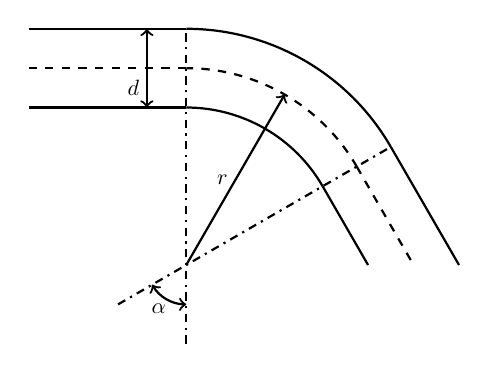
\begin{tikzpicture}[ scale=1, every node/.style={scale=0.8},] 
\draw[thick, dash dot] (0,-1) -- (0,3);
\draw[thick, dash dot] (-0.866,-0.5) -- (2.598,1.5);
% Inlet pipe
\draw[thick] (0,2) -- (-2,2);
\draw[thick, dashed] (0,2.5) -- (-2,2.5);
\draw[thick] (0,3) -- (-2,3);
% Bend
\draw[thick] (1.732,1) arc (30:90:2);
\draw[thick, dashed] (2.165,1.25) arc (30:90:2.5);
\draw[thick] (2.598,1.5) arc (30:90:3);
% Outlet pipe
\draw[thick] (1.732,1) -- (2.309,0);
\draw[thick, dashed] (2.165,1.25) -- (2.887,0);
\draw[thick] (2.598,1.5) -- (3.464,0);
% Annotations
\node[anchor=east] at (-0.5,2.25) {$d$};
\draw[thick, <->] (-0.5,2) -- (-0.5,3);
\draw[thick, <->] (-0.433,-0.25) arc (30:90:-0.5);
\node[anchor=north] at (-0.35,-0.39) {$\alpha$};
\draw[thick, ->] (0,0) -- (1.25,2.165);
\node[anchor=east] at (0.625,1.082) {$r$};
\end{tikzpicture} 
\caption{A bend in a pipe of diameter $d$ with a bend radius $r$ and bend angle $\alpha$.}
\label{fig:bend_diagram}
\end{figure}
\subsubsection{Size changes}

Flow through contractions/expansions cause the flow to accelerate/decelerate so it is important to consider size changes when pipes of different diameter are connected. Contractions and expansions are really two sides of the same coin, a contraction with flow in the opposite direction is an expansion just as an expansion with reverse flow is a contraction. Lets consider contractions and expansions separately before their action with reverse flow and combining them into a single component.  

\paragraph{Contraction}

Let us consider a contraction where the flow is from inlet node $i$ to outlet node $k$, as shown in figure \ref{fig:contraction_diagram}. The head loss due to the contraction \cite{rennels22} is given by
\begin{align}
H_L = \frac{K_c V_i^2}{2g},
\end{align}
where the contraction loss coefficient is
\begin{align*}
K_c = 0.0696 \left( 1 - \beta^2 \right) \lambda^2 + \left( \lambda - 1 \right)^2
\end{align*}
and
\begin{align*}
\lambda = 1 + 0.622 \left( 1 - 0.215 \beta^2 - 0.785 \beta^5 \right).
\end{align*}
Here $\beta = d_k / d_i$ is the ratio of the smaller diameter to the larger diameter and $V_i = Q_j / A_i$ is the inlet flow velocity. 

\begin{figure}
\centering
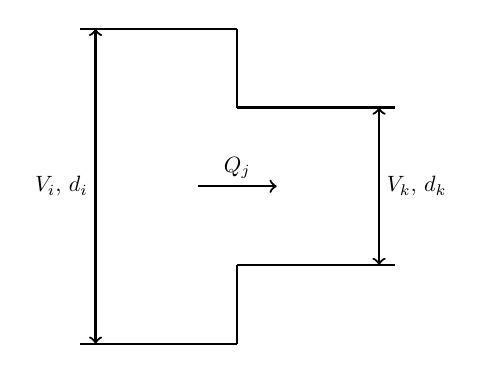
\begin{tikzpicture}[ scale=1, every node/.style={scale=0.8},] 
% Inlet pipe
\draw[thick] (0,0) -- (-2,0);
\draw[thick] (0,4) -- (-2,4);
% Contraction
\draw[thick] (0,0) -- (0,1);
\draw[thick] (0,4) -- (0,3);
% Outlet pipe
\draw[thick] (0,1) -- (2,1);
\draw[thick] (0,3) -- (2,3);
% Annotations
\node[anchor=east] at (-1.8,2) {$V_i$, $d_i$};
\draw[thick, <->] (-1.8,0) -- (-1.8,4);
\node[anchor=south] at (0,2) {$Q_j$};
\draw[thick, ->] (-0.5,2) -- (0.5,2);
\node[anchor=west] at (1.8,2) {$V_k$, $d_k$};
\draw[thick, <->] (1.8,1) -- (1.8,3);
\end{tikzpicture} 
\caption{An abrupt contraction where positive flow is from $i$ to $k$. The size ratio is $\beta = d_k / d_i$.}
\label{fig:contraction_diagram}
\end{figure}

\paragraph{Expansion}

For an expansion where the flow is from inlet node $i$ to outlet node $k$, as shown in figure \ref{fig:expansion_diagram} the head loss due to the expansion \cite{rennels22} is given by
\begin{align}
H_L = \frac{\hat{K}_e V_i^2}{2g},
\end{align}
where
\begin{align*}
\hat{K}_e = \left(1 - \hat{\beta}^2 \right)^2
\end{align*}
and $\hat{\beta} =  d_i / d_k$.

\begin{figure}
\centering
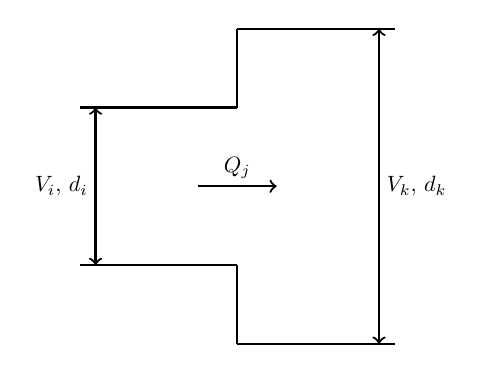
\begin{tikzpicture}[ scale=1, every node/.style={scale=0.8},] 
% Outlet pipe
\draw[thick] (0,0) -- (2,0);
\draw[thick] (0,4) -- (2,4);
% Contraction
\draw[thick] (0,0) -- (0,1);
\draw[thick] (0,4) -- (0,3);
% Inlet pipe
\draw[thick] (0,1) -- (-2,1);
\draw[thick] (0,3) -- (-2,3);
% Annotations
\node[anchor=west] at (1.8,2) {$V_k$, $d_k$};
\draw[thick, <->] (1.8,0) -- (1.8,4);
\node[anchor=south] at (0,2) {$Q_j$};
\draw[thick, ->] (-0.5,2) -- (0.5,2);
\node[anchor=east] at (-1.8,2) {$V_i$, $d_i$};
\draw[thick, <->] (-1.8,1) -- (-1.8,3);
\end{tikzpicture} 
\caption{An abrupt expansion where positive flow is from $i$ to $k$. The size ratio is $\hat{\beta} = d_i / d_k$.}
\label{fig:expansion_diagram}
\end{figure}

\paragraph{Reverse flow}

For positive flows, $Q_j > 0$, if $\beta < 1$ or $\hat{\beta} > 1$ then we have a contraction but if $\beta > 1$ or $\hat{\beta} < 1$ then we have an expansion. For negative flows, $Q_j < 0$, the situation is reversed if $\beta < 1$ or $\hat{\beta} > 1$ then we have an expansion but if $\beta > 1$ or $\hat{\beta} < 1$ then we have a contraction.

Reverse flow in a contraction, see figure \ref{fig:contraction_diagram}, is actually an expansion with a head loss given by
\begin{align}
H_L = \frac{K_e V_k^2}{2g},
\end{align}
where
\begin{align*}
K_e = \left(1 - \beta^2 \right)^2.
\end{align*}

Similarly reverse flow in an expansion, see figure \ref{fig:expansion_diagram}, is actually a contraction with a head loss given by
\begin{align}
H_L = \frac{\hat{K}_c V_k^2}{2g},
\end{align}
where 
\begin{align*}
\hat{K}_c = 0.0696 \left( 1 - \hat{\beta}^2 \right) \hat{\lambda}^2 + \left( \hat{\lambda} - 1 \right)^2
\end{align*}
and
\begin{align*}
\hat{\lambda} = 1 + 0.622 \left( 1 - 0.215 \hat{\beta}^2 - 0.785 \hat{\beta}^5 \right).
\end{align*}

\paragraph{Resistance for abrupt size changes}

These four different scenarios for forward/reverse flow and $\beta = \hat{\beta}^{-1}$ greater/less than $1$ means the resistance term for an abrupt size changes must be split into four parts. 
\begin{align}\label{abrupt_size_change_resistance}
\boxed{
  \!\begin{gathered}
  R_j = -\frac{K Q_j^2}{2 A} + g A \Delta H_j, \hspace{0.5cm} \text{where} \\
A = \begin{cases}
A_i &\text{if} \hspace{0.5cm} Q_j > 0,\\
A_k &\text{if} \hspace{0.5cm} Q_j < 0,
\end{cases} \nonumber \\
K = \begin{cases} 
K_c, &\text{if} \hspace{0.5cm} Q_j > 0, \beta < 1, \\
\hat{K}_e, &\text{if} \hspace{0.5cm} Q_j > 0, \beta > 1, \\
K_e, &\text{if} \hspace{0.5cm} Q_j < 0, \beta < 1, \\
\hat{K}_c, &\text{if} \hspace{0.5cm} Q_j < 0, \beta > 1.
\end{cases} \nonumber
  \end{gathered}
}
\end{align}

\subsubsection{Open pipes}

\subsubsection{Sprinklers}

\subsubsection{Flow controllers}

\subsubsection{Tee junctions}

\subsubsection{Cross junctions}

{\color{red} ETC -> other devices i.e. surge tanks, reservoirs, safety relief valve}

The solution of the steady state problem for flow networks has been thoroughly explored and many other solution methods exist. It is illustrative to see how the water-hammer equations collapse to the steady state problem in the absence of time variation but we must continue towards our original goal, to devise a method for calculating fluid transients in pipe networks. 

{\color{red} Appendix on calculating the laminar initial guess.}


\section{Transient solver} \label{sec:transient_solver}

The full transient equations are more difficult to solve than the steady state problem as the resistance term in the momentum is now time dependent and we must retain all the terms in the discrete continuity equation \eqref{discrete_continuity_eqn}. The equations must be stepped forward in time using a scheme which is both accurate and numerically stable. 

\subsection{Theta method}

The $\theta$-method is a generalisation of the Crank-Nicolson method which allows the scheme to be made more or less implicit. In general the scheme takes the form
\begin{align}
\frac{u_i^{n+1} - u_i^{n}}{\Delta t} = \theta F_i^{n+1}\left(u,x,t,\pardiv{}{u}{x},\ldots \right) + (1-\theta) F_i^{n}\left(u,x,t,\pardiv{}{u}{x},\ldots \right),
\end{align}
where $\theta \in [0,1]$. If $\theta = 0$ then the scheme is the explicit forward Euler method, if $\theta = 1$ then it is the fully implicit backward Euler method and if $\theta = 1/2$ then it is the Crank-Nicolson method. Usually the Crank-Nicolson scheme is preferred to both the forward and backward Euler methods as it is second order accurate whereas they are both only first order accurate. However the approximate solutions found using the Crank-Nicolson scheme sometimes include spurious oscillations so it may be preferable to use the less accurate implicit scheme in certain situations.


Using the $\theta$-method on the continuity equation \eqref{discrete_continuity_eqn} we have
\begin{align}
\mathbf{K}^T \left( \theta \mathbf{Q}^{n+1} + (1-\theta)\mathbf{Q}^{n} \right) + \mathbf{D} \left( \frac{\mathbf{H}^{n+1} - \mathbf{H}^{n}}{\Delta t} \right) = \mathbf{C}.
\end{align}
Then for the momentum equation \eqref{discrete_momentum_eqn} we have
\begin{align}
\mathbf{B} \frac{\mathbf{Q}^{n+1} - \mathbf{Q}^{n}}{\Delta t} = \mathbf{R}\left( \theta \mathbf{Q}^{n+1} + (1-\theta)\mathbf{Q}^{n}, \theta \mathbf{K} \mathbf{H}^{n+1} + (1-\theta) \mathbf{K} \mathbf{H}^n \right).
\end{align}
At time-step $n$ the pipe flow rates $\mathbf{Q}^{n}$ and nodal heads $\mathbf{H}^{n}$ are known and we would like to estimate the solution at the subsequent time-step $n+1$. The steady state solution $\mathbf{Q}^{0}$ and $\mathbf{H}^{0}$ is used to initialise the scheme.

\subsubsection{Newton iteration} 

Since the solution is known at time-step $n$ only the solution at time-step $n+1$ needs to be split into a known/guessed part and a correction i.e. $\mathbf{Q}^{n+1} = \mathbf{Q}^{n+1,g} + \mathbf{Q}^{n+1,c}$ and $\mathbf{H}^{n+1} = \mathbf{H}^{n+1,g} + \mathbf{H}^{n+1,c}$. The resitance term is then approximated as
\begin{align*}
\mathbf{R}(\mathbf{Q}, \mathbf{K} \mathbf{H}) \approx \mathbf{R}\left(\bar{\mathbf{Q}}, \mathbf{K} \bar{\mathbf{H}} \right) + \pardiv{}{\mathbf{R}}{\mathbf{Q}} \Bigg\vert_{\bar{\mathbf{Q}}} \theta \mathbf{Q}^{n+1,c} + \pardiv{}{\mathbf{R}}{\mathbf{K} \mathbf{H}} \Bigg\vert_{\mathbf{K} \bar{\mathbf{H}}} \theta \mathbf{K} \mathbf{H}^{n+1,c},
\end{align*}
where $\bar{\mathbf{Q}}=\theta \mathbf{Q}^{n+1,g} + (1-\theta) \mathbf{Q}^{n}$, $\bar{\mathbf{H}}=\theta \mathbf{H}^{n+1,g} + (1-\theta) \mathbf{H}^{n}$. Splitting into a known part and correction at the next time step the continuity equation is given by
\begin{align}\label{discrete_transient_continuity_eqn_newton}
\theta \mathbf{K}^T \mathbf{Q}^{n+1,c} + \frac{1}{\Delta t} \mathbf{D} \mathbf{H}^{n+1,c} = \mathbf{C} - \mathbf{K}^T \bar{\mathbf{Q}} - \frac{1}{\Delta t} \mathbf{D} \left( \mathbf{H}^{n+1,g} - \mathbf{H}^{n} \right),
\end{align}
and the momentum equation is given by
\begin{align}\label{discrete_transient_momentum_eqn_newton}
\left(\frac{1}{\Delta t} \mathbf{B} - \theta \pardiv{}{\mathbf{R}}{\mathbf{Q}} \Bigg\vert_{\bar{\mathbf{Q}}} \right) \mathbf{Q}^{n+1,c} - \theta \pardiv{}{\mathbf{R}}{\mathbf{K} \mathbf{H}} \Bigg\vert_{\mathbf{K} \bar{\mathbf{H}}} \mathbf{K} \mathbf{H}^{n+1,c} = \mathbf{R}\left(\bar{\mathbf{Q}}, \mathbf{K} \bar{\mathbf{H}} \right) - \frac{1}{\Delta t} \left(\mathbf{Q}^{n+1,g} - \mathbf{Q}^{n} \right).
\end{align} 
Equations \eqref{discrete_transient_continuity_eqn_newton} and \eqref{discrete_transient_momentum_eqn_newton} must be solved together as the single system of equations
\begin{align}\label{discrete_transient_system}
\begin{bmatrix}
\theta \mathbf{K}^T & \frac{1}{\Delta t}\mathbf{D} \\
\frac{1}{\Delta t}\mathbf{B}-\theta \bar{\mathbf{J}} & - \theta \bar{\mathbf{G}}
\end{bmatrix} 
\begin{bmatrix}
\mathbf{Q}^{n+1,c} \\ \mathbf{H}^{n+1,c}
\end{bmatrix} = \begin{bmatrix}
\mathbf{C} - \mathbf{K}^T \bar{\mathbf{Q}} - \frac{1}{\Delta t} \mathbf{D} \left( \mathbf{H}^{n+1,g} - \mathbf{H}^{n} \right) \\
\mathbf{R}\left(\bar{\mathbf{Q}}, \mathbf{K} \bar{\mathbf{H}} \right) - \frac{1}{\Delta t} \left(\mathbf{Q}^{n+1,g} - \mathbf{Q}^{n} \right)
\end{bmatrix},
\end{align}
where $\bar{\mathbf{J}} = \pardiv{}{\mathbf{R}}{\mathbf{Q}} \big\vert_{\bar{\mathbf{Q}}}$ and $\bar{\mathbf{G}} = \pardiv{}{\mathbf{R}}{\mathbf{K} \mathbf{H}} \big\vert_{\mathbf{K} \bar{\mathbf{H}}} \mathbf{K} $. In a similar manner to the steady solver the system of equations \eqref{discrete_transient_system} would be solved for the corrections, $\mathbf{Q}^{n+1,c}$ and $\mathbf{H}^{n+1,c}$, these would then be used to update the guess $\mathbf{Q}^{n+1,g} \rightarrow \mathbf{Q}^{n+1,g} + \mathbf{Q}^{n+1,c} $ and $\mathbf{H}^{n+1,g} \rightarrow \mathbf{H}^{n+1,g} + \mathbf{H}^{n+1,c} $ and then the process would be repeated until the corrections are sufficiently small. After updating the simulation time $t \rightarrow t + \Delta t$, this time-stepping is repeated until the simulation is complete.   

\subsection{Boundary conditions}

Boundary conditions may be applied at the nodes in the system by replacing the continuity equation at that node with an appropriate boundary condition. For example if the head is specified to be $H_{known}$ at a given node $i$ then we have the condition 
\begin{align}
\theta H_i^{n+1,c} = H_{known} - \left( \theta H_i^{n+1,g} + (1-\theta)H_i^n \right),
\end{align} 
which can be used to replace row $i$ in the system of equations \eqref{discrete_transient_system}. Here the boundary head $H_{known}$ may vary over time. Known flow rates at the nodes are specified using the consumption vector $\mathbf{C}$. The consumption vector $\mathbf{C}$ in the system of equations may also vary with time. 

\subsubsection{Surge tanks}

A surge tank is an open topped vessel, filled with fluid upto some predetermined height, as shown in figure \ref{fig:surge_tank_diagram}. By damping the pressure response and supplying/storing fluid a surge tank is often able to alleviate the ill effects of transient flows in a system {\color{red} Reference Chaudry p349-350}. Surge tanks are able to be modelled by modifying the consumption term in the continuity equation at a node thereby modifying the rate at which the nodal head changes with time. 

\begin{figure}
\centering
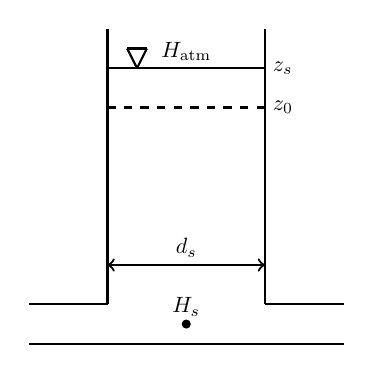
\begin{tikzpicture}[ scale=1, every node/.style={scale=0.8},] 
% Pipe
\draw[thick] (2,0) -- (-2,0);
\draw[thick] (1,0.5) -- (2,0.5);
\draw[thick] (-1,0.5) -- (-2,0.5);
% Sides
\draw[thick] (1,0.5) -- (1,4);
\draw[thick] (-1,0.5) -- (-1,4);
% Water levels
\draw[thick, dashed] (1,3) -- (-1,3);
\draw[thick] (1,3.5) -- (-1,3.5);


% Annotations
\node[anchor=west] at (1,3.5) {$z_s$};
\node[anchor=west] at (1,3) {$z_0$};
\node[anchor=south] at (0,1) {$d_s$};
\draw[thick, <->] (1,1) -- (-1,1);

% Node labels
\draw[fill=black] (0,0.25) circle (0.05cm);
\node[anchor=south] at (0,0.25) {$H_s$};
%\draw[fill=black] (0,3.5) circle (0.05cm);
\node[anchor=south] at (0,3.5) {$H_{\text{atm}}$};
% Free surface symbol
\draw[thick] (-0.5,3.75) -- (-0.75,3.75);
\draw[thick] (-0.5,3.75) -- (-0.625,3.5);
\draw[thick] (-0.75,3.75) -- (-0.625,3.5);
\end{tikzpicture} 
\caption{A surge tank boundary at node $s$ with an a fluid level $z_s$, an initial fluid level $z_0$ and tank diameter $d_s$.}
\label{fig:surge_tank_diagram}
\end{figure}

Suppose that a surge tank is placed in the network at node $s$, at this node we have the continuity equation
\begin{align}
\left( \mathbf{K}^T \right)_s \mathbf{Q} + D_{s,s} \pardiv{}{H_s}{t} = C_s,
\end{align}
where $\left( \mathbf{K}^T \right)_s$ indicates the $s$th row of the matrix $\mathbf{K}^T$ and $D_{s,s}$ indicates the element of the matrix $D$ at row $s$ and column $s$. The flow which leaves the node and fills the surge tank may be modelled by choosing an appropriate expression for the consumption term $C_s$. 

The nodal head $H_s$ is equal to the head due to atmospheric pressure plus the fluid column height i.e.
\begin{align}
H_s = H_{\text{atm}} + z_s.
\end{align} 
The rate at which fluid flows into the surge tank is
\begin{align*}
A_s \frac{d z_s}{d t},
\end{align*}
where $A_s = \pi d_s^2 / 4$ is the cross-sectional area of the tank. If we assume that the fluid in the tank moves as a slug then we may say that
 \begin{align*}
A_s \frac{d z_s}{d t} = A_s \pardiv{}{z_s}{t} = A_s \pardiv{}{H_s}{t}.
\end{align*}
Therefore, since flow into the tank is equal to flow out of the node $(C_s < 0)$, we may rewrite the continuity equation as
\begin{align*}
\left( \mathbf{K}^T \right)_s \mathbf{Q} + D_{s,s} \pardiv{}{H_s}{t} = - A_s \pardiv{}{H_s}{t}.
\end{align*}
Splitting into a known part and correction at the next time step the continuity equation, at node $s$, is given by
\begin{align}\label{discrete_transient_continuity_eqn_surge}
\theta \left( \mathbf{K}^T \right)_s \mathbf{Q}^{n+1,c} + \frac{(D_{s,s} + A_s)}{\Delta t} H_s^{n+1,c} = - \left( \mathbf{K}^T \right)_s \bar{\mathbf{Q}} - \frac{(D_{s,s} + A_s)}{\Delta t} \left( H_s^{n+1,g} - H_s^{n} \right).
\end{align}
The equation \eqref{discrete_transient_continuity_eqn_surge} then substitutes the $s$th row of the system of governing equations \eqref{discrete_transient_system}. It may be observed that by adding the surge tank we are effectively modifying the coefficient $D_{s,s}$ such that $D_{s,s} \rightarrow D_{s,s} + A_s$ thereby reducing the rate at which $H_s$ changes with time for a given set of flow rates through the edges connected to node $s$. 


\subsection{Components}

Components other than pipes may be specified in equation \eqref{discrete_momentum_eqn}. For a general component, of the form shown in figure \ref{fig:general_component}, a relationship between the nodal heads and the pipe flow rate must be specified. 

\begin{figure}
\centering
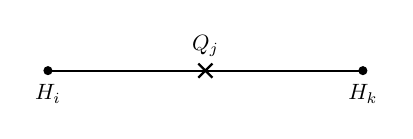
\begin{tikzpicture}[scale=1, every node/.style={scale=0.8}] 
%\draw[step=1cm,color=gray] (3,0) grid (7,3);
\node[anchor=north] at (3,-0.08) {$H_i$};
\draw[fill=black] (3,0) circle (0.05cm);
\node[anchor=south] at (5,0.08) {$Q_j$};
\draw[thick] (5,0) node[cross=4pt] {};
\node[anchor=north] at (7,-0.08) {$H_k$};
\draw[fill=black] (7,0) circle (0.05cm);
\draw[thick] (3,0) -- (7,0);
\end{tikzpicture} 
\caption{General component $j$ with an average flow rate $Q_j$ and nodal heads $H_i$ and $H_k$.}
\label{fig:general_component}
\end{figure}

% Transient components

%{\color{red}

\subsubsection{Reservoir}

For example a reservoir with an entrance loss 
\begin{align}
h_e = \frac{C_e Q^2}{2 g A^2},
\end{align}
where $C_e$ is the entrance loss coefficient, has resistance term
\begin{align}\label{reservoir_resistance}
R_j =& \frac{(C_e)_j Q_j^2}{2 g A_j^2} \\
\approx & \frac{(C_e)_j }{2 g A_j^2} \left[ \bar{Q}_j^2 + 2 \theta \bar{Q}_j Q_j^{n+1,c}  \right],
\end{align}
where $\bar{Q} = \theta Q_j^{n+1,g} + (1-\theta) Q_j^n$. So if the reservoir boundary is located at node $i$ then we replace the $i$-th contnuity equation with 
\begin{align}
\theta H_i^{n+1,c} = H_{res} - \bar{H}_i
\end{align}
and replace the resistance term in the momentum equation \eqref{discrete_momentum_eqn} with \eqref{reservoir_resistance} and set $L_j = 0$ in $\mathbf{B}$.

}

\subsubsection{Valves}

Transient flows in pipe networks may be caused by the closing and opening of valves. In order to describe the transient behaviour of a valves we must define the valve open ratio $\tau(t)$ as a function of time. The valve open percentage is then used to determine the loss coefficient $k$ in the valve resistance equation \eqref{valve_resistance}.

\paragraph{Closing}
 
 The function $\tau(t)$, as shown in figure \ref{fig:valve_closing}, for a valve closure is given by 
\begin{align}\label{valve_closure_function}
\tau(t) = 
\begin{cases} 
\tau_{steady}, &\text{if} \hspace{0.5cm} t \leq t_e \\
\tau_{steady} \left( 1 - \frac{t-t_e}{t_c} \right)^m, &\text{if} \hspace{0.5cm} t_e \leq t \leq t_e + t_c \\
0, &\text{if} \hspace{0.5cm} t \geq t_e + t_c, 
\end{cases}
\end{align} 
where $t_e$ is the event time, $t_c$ is the time taken for the valve to close, $\tau_{steady}$ is the steady state valve open percentage. The exponent $m > 0$ modifies the shape of the closure profile with $m=1$ corresponding to a linear profile. 
 
\begin{figure}
\centering
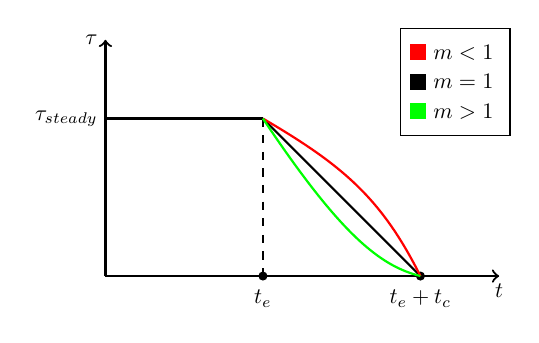
\begin{tikzpicture}[
	scale=1, 
	every node/.style={scale=0.8},
	greennode/.style={shape=rectangle, fill=green, draw=green, minimum size =0.01cm},
	rednode/.style={shape=rectangle, fill=red, draw=red, minimum size =0.01cm},
	blacknode/.style={shape=rectangle, fill=black, draw=black, minimum size =0.01cm},
] 
\draw[thick, ->] (0,0) -- (0,3);
\node[anchor=east] at (0,3) {$\tau$};
\draw[thick, ->] (0,0) -- (5,0);
\node[anchor=north] at (5,0) {$t$};
\node[anchor=north] at (2,-0.08) {$t_e$};
\draw[fill=black] (2,0) circle (0.05cm);
\node[anchor=north] at (4,-0.08) {$t_e + t_c$};
\draw[fill=black] (4,0) circle (0.05cm);
\node[anchor=east] at (0,2) {$\tau_{steady}$};
\draw[thick] (0,2) -- (2,2);
\draw[thick] (2,2) -- (4,0);
\draw[thick, dashed] (2,2) -- (2,0);
\draw[thick, red] (2,2) .. controls (3,1.414) and (3.5,1) .. (4,0);
\draw[thick, green] (2,2) .. controls (3,0.5) and (3.5,0.125) .. (4,0);

\matrix [draw,below left] at (current bounding box.north east) {
  \node [rednode,label=right: {$m < 1$}] {}; \\
  \node [blacknode,label=right: {$m = 1$}] {}; \\
  \node [greennode,label=right: {$m > 1$}] {}; \\
};
\end{tikzpicture} 
\caption{Valve closure. The open ratio $\tau(t)$ goes from $\tau_{steady}$ at time $t_e$ to zero at time $t_e + t_c$, where $t_c$ is the time taken for the valve to close. The exponent $m$ modifies the closure profile, as shown by the red and green curves.}
\label{fig:valve_closing}
\end{figure}

\paragraph{Opening}

{\color{red} TODO Valve opening}

\subsubsection{Pumps}

The starting and stopping of pumps are a significant cause of transient flows in pumping systems. Starting of a pump is usually controlled by keeping the discharge valve close until the pump reaches the rated speed and then slowly opening the valve. However sometimes pumps are started without using valves by controlling the speed electronically. Similarly pump shutdown may be assisted by valve closure or by external control. Another common source of pump transients is power failure, in this situation the speed of the pump is no longer controlled and is instead determined by the torque on the pump and the flow conditions.  

\paragraph{Shutdown}

The simplest way to shutdown a pump in a controlled manner is a reduction of the rotational speed, at a specified event time $t_e$, to zero at time $t_e + t_c$, where $t_c$ is stopping time. The rotational speed $N$ as a function of time $t$, as shown in figure \ref{fig:pump_shutdown}, is defined by the piecewise function
\begin{align}\label{pump_shutdown_function}
N(t) = 
\begin{cases} 
N_{steady}, &\text{if} \hspace{0.5cm} t \leq t_e \\
N_{steady} \left( 1 - \frac{t-t_e}{t_c} \right)^m, &\text{if} \hspace{0.5cm} t_e \leq t \leq t_e + t_c \\
0, &\text{if} \hspace{0.5cm} t \geq t_e + t_c. 
\end{cases}
\end{align}
The exponent $m > 0$ modifies the shape of the closure profile with $m=1$ corresponding to a linear profile. Changing the rotational speed alters both $n$ and $\theta$ in the pump resistance equation \eqref{pump_resistance} so that the resistance varies with time too. 

\begin{figure}
\centering
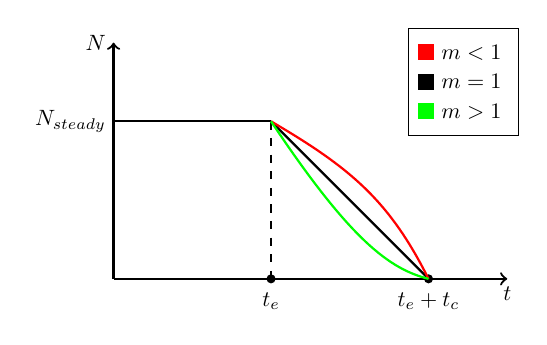
\begin{tikzpicture}[
	scale=1, 
	every node/.style={scale=0.8},
	greennode/.style={shape=rectangle, fill=green, draw=green, minimum size =0.01cm},
	rednode/.style={shape=rectangle, fill=red, draw=red, minimum size =0.01cm},
	blacknode/.style={shape=rectangle, fill=black, draw=black, minimum size =0.01cm},
] 
\draw[thick, ->] (0,0) -- (0,3);
\node[anchor=east] at (0,3) {$N$};
\draw[thick, ->] (0,0) -- (5,0);
\node[anchor=north] at (5,0) {$t$};
\node[anchor=north] at (2,-0.08) {$t_e$};
\draw[fill=black] (2,0) circle (0.05cm);
\node[anchor=north] at (4,-0.08) {$t_e + t_c$};
\draw[fill=black] (4,0) circle (0.05cm);
\node[anchor=east] at (0,2) {$N_{steady}$};
\draw[thick] (0,2) -- (2,2);
\draw[thick] (2,2) -- (4,0);
\draw[thick, dashed] (2,2) -- (2,0);
\draw[thick, red] (2,2) .. controls (3,1.414) and (3.5,1) .. (4,0);
\draw[thick, green] (2,2) .. controls (3,0.5) and (3.5,0.125) .. (4,0);

\matrix [draw,below left] at (current bounding box.north east) {
  \node [rednode,label=right: {$m < 1$}] {}; \\
  \node [blacknode,label=right: {$m = 1$}] {}; \\
  \node [greennode,label=right: {$m > 1$}] {}; \\
};
\end{tikzpicture} 
\caption{Pump shutdown. The rotational speed $N(t)$ goes from $N_{steady}$ at time $t_e$ to zero at time $t_e + t_c$, where $t_c$ is the time taken for the pump to stop. The exponent $m$ modifies the closure profile, as shown by the red and green curves.}
\label{fig:pump_shutdown}
\end{figure}

\paragraph{Startup}

The time varying function describing the startup of a pump, as shown in figure \ref{fig:pump_startup}, is very similar to the function describing a shutdown and is given by 

\begin{align}\label{pump_startup_function}
N(t) = 
\begin{cases} 
0, &\text{if} \hspace{0.5cm} t \leq t_e \\
N_{\infty} \left( \frac{t-t_e}{t_s} \right)^m, &\text{if} \hspace{0.5cm} t_e \leq t \leq t_e + t_s \\
N_{\infty}, &\text{if} \hspace{0.5cm} t \geq t_e + t_s, 
\end{cases}
\end{align}
where again $t_e$ is the event time, $t_s$ is startup time and $N_{\infty}$ is the pump speed once the startup procedure has been completed. The exponent $m > 0$ modifies the shape of the closure profile with $m=1$ corresponding to a linear profile. 


\begin{figure}
\centering
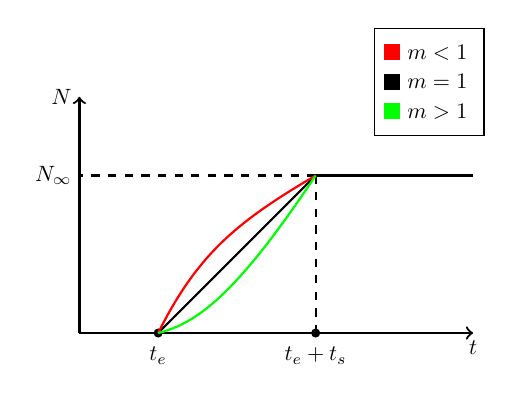
\begin{tikzpicture}[
	scale=1, 
	every node/.style={scale=0.8},
	greennode/.style={shape=rectangle, fill=green, draw=green, minimum size =0.01cm},
	rednode/.style={shape=rectangle, fill=red, draw=red, minimum size =0.01cm},
	blacknode/.style={shape=rectangle, fill=black, draw=black, minimum size =0.01cm},
] 
\draw[thick, ->] (0,0) -- (0,3);
\node[anchor=east] at (0,3) {$N$};
\draw[thick, ->] (0,0) -- (5,0);
\node[anchor=north] at (5,0) {$t$};
\node[anchor=north] at (1,-0.08) {$t_e$};
\draw[fill=black] (1,0) circle (0.05cm);
\node[anchor=north] at (3,-0.08) {$t_e + t_s$};
\draw[fill=black] (3,0) circle (0.05cm);
\node[anchor=east] at (0,2) {$N_{\infty}$};

\draw[thick] (3,2) -- (5,2);
\draw[thick] (1,0) -- (3,2);
\draw[thick, dashed] (3,2) -- (3,0);
\draw[thick, dashed] (3,2) -- (0,2);
\draw[thick, red] (1,0) .. controls (1.5,1) and (2,1.414)  .. (3,2);
\draw[thick, green] (1,0) .. controls (1.5,0.125) and (2,0.5) .. (3,2);

\matrix [draw,left] at (current bounding box.north east) {
  \node [rednode,label=right: {$m < 1$}] {}; \\
  \node [blacknode,label=right: {$m = 1$}] {}; \\
  \node [greennode,label=right: {$m > 1$}] {}; \\
};
\end{tikzpicture} 
\caption{Pump startup. The rotational speed $N(t)$ goes from zero at time $t_e$ to $N_{\infty}$ at time $t_e + t_s$, where $t_s$ is the time taken for the pump to startup. The exponent $m$ modifies the closure profile, as shown by the red and green curves.}
\label{fig:pump_startup}
\end{figure}

% \paragraph{General speed variation (piecewise linear)}

% \paragraph{Power failure}

\subsubsection{Relief valves}

\paragraph{Pressure relief valves}

\paragraph{Safety valves}

\subsubsection{Check / Non-return valves}

A check or non-return valve is a valve that allows fluid to flow through it in one direction only. \ 
The resistance of a check valve has the same form as for a standard valve, see equation \ 
\eqref{valve_resistance}, however the inverse loss coefficient $k_j^{-1}$ is given by
\begin{align}
    \boxed{ 
        k_j^{-1} = 
        \begin{cases}
            0, & \text{if } \Delta H_j \leq 0, \\
            k_0^{-1}, & \text{if } \Delta H_j > 0.
        \end{cases}
    }
\end{align}
This means that the check valve is open when the pressure difference across it is positive and \ 
closed when the pressure difference is negative. The value $k_0$ is the loss coefficient of the \ 
valve when it is fully open. For steady flow, the check valve is considered to be open \ 
$(\tau = 1)$, so the inverse loss coefficient is $k_0^{-1}$. 



\begin{thebibliography}{9}
\bibitem{chaudhry14} Chaudhry, M.H., 2014. Applied hydraulic transients.

\bibitem{ellis01} Ellis, D.J., 2001. The behaviour of pipe network analysis solution techniques/by David J. Ellis (Doctoral dissertation).

\bibitem{grady10} Grady, L.J. and Polimeni, J.R., 2010. Discrete calculus: Applied analysis on graphs for computational science. Springer Science \& Business Media.

\bibitem{rennels22} Rennels, D.C., 2022. Pipe flow: A practical and comprehensive guide. John Wiley \& Sons.

\bibitem{streeter78} Wylie, E.B. and Streeter, V.L., 1978. Fluid transients. New York.

\end{thebibliography}

\end{document}
